\documentclass[autodetect-engine,dvipdfmx-if-dvi,ja=standard,a4j,jbase=11pt,magstyle=nomag*]{bxjsreport}
% \documentclass[uplatex, dvipdfmx, a4paper, 11ptj, report]{jsbook}
% small japanese font size:     9pt, 10pt, 11pt, 12pt, 14pt, ... (please refer the document of jsclasses)
% word-like japanese font size: 10ptj 10.5ptj, 11ptj, 12ptj (or jbase=xxpt (without 'j') if error is occured)

\usepackage{ifptex,ifxetex,ifluatex}
\ifluatex
    \usepackage{bxcalcux}
    \ltjsetparameter{jacharrange={-2,-3}}
    \usepackage{luatexja-otf}
    \usepackage{bxbase}
\else\ifxetex
    % \usepackage{zxjatype}
    % \usepackage[macros]{zxotf}
    \XeTeXgenerateactualtext=1
    \usepackage{xltxtra}
    \usepackage{bxbase}
\else\ifuptex
    \usepackage{otf}
    \usepackage[prefernoncjk]{pxcjkcat}
    \cjkcategory{sym11,sym18,sym19}{cjk}
    \usepackage[utf8]{inputenc}
    \usepackage{pxbase}
\else\ifstrictptex
    \usepackage{otf}
    \usepackage[utf8]{inputenc}
    \usepackage{pxbase}
\fi\fi\fi\fi

\usepackage[LGR,T2A,T1]{fontenc}

\usepackage{graphicx}
% \usepackage[dvipdfmx]{graphicx}
\usepackage{grffile}

% paper layout setting
\setpagelayout{noheadfoot, left=18.0truemm, right=18.0truemm, top=29.0truemm, bottom=26.0truemm, columnsep=6.5truemm}
% \setpagelayout{noheadfoot, left=15.0truemm, right=5.0truemm, top=12.5truemm, bottom=12.5truemm, columnsep=5.0truemm}

% font setting
\usepackage{amsmath}
\usepackage{amssymb}
\usepackage{mathtools}
\usepackage{bm}
\usepackage{fix-cm}
\usepackage{newtxtext}
\usepackage[slantedGreek]{newtxmath}

% caption setting
\usepackage[font=bf,labelfont=bf,labelsep=quad]{caption}

% to balance the last page of the two-column article
% \usepackage[nospread, keeplastbox, nodebug]{flushend}

% title font style
\renewcommand{\headfont}{\bfseries}

% section setting (using titlesec, uelm package)
\renewcommand{\thesection}{\arabic{section}}
\renewcommand{\thesubsection}{\arabic{section}.\arabic{subsection}}

\usepackage[explicit]{titlesec}
\usepackage[normalem]{ulem}
\titleformat{name=\section}{\normalfont\headfont\normalsize\raggedright}{}{0pt}{\uline{\thesection.\quad#1}}
\titleformat{name=\section,numberless}{\normalfont\headfont\normalsize\raggedright}{}{0pt}{\uline{#1}}
% \titleformat{name=\section}{\normalfont\headfont\normalsize\raggedright}{}{0pt}{\thesection.\quad#1}
\titlespacing{name=\section}{0pt}{.5\Cvs plus .0\Cvs minus .3\Cvs}{.1\Cvs plus .0\Cvs minus .1\Cvs}
\titleformat{name=\subsection}{\normalfont\headfont\normalsize\raggedright}{}{0pt}{\thesubsection.\quad#1}
\titleformat{name=\subsection,numberless}{\normalfont\headfont\normalsize\raggedright}{}{0pt}{#1}
\titlespacing{name=\subsection}{0pt}{.3\Cvs plus .0\Cvs minus .2\Cvs}{.0\Cvs plus .0\Cvs minus .0\Cvs}

% \makeatletter
% \renewcommand{\section}{\@startsection{section}{1}{\z@}{.5\baselineskip}{.1\baselineskip}{\normalfont\normalsize\headfont\raggedright}}
% \renewcommand{\subsection}{\@startsection{subsection}{2}{\z@}{.3\baselineskip}{\z@}{\normalfont\normalsize\headfont\raggedright}}
% \makeatother

\usepackage{secdot}
\sectiondot{section}
\sectiondot{subsection}

% list (itemize, enumerate, description, ...)
\usepackage{enumitem}
\setlist[1]{parsep=.0\baselineskip,topsep=.2\baselineskip,itemsep=.1\baselineskip}
% \makeatletter
% \def\@listi{\leftmargin\leftmargini
%     \parsep \z@
%     \topsep .2\baselineskip
%     \itemsep .1\baselineskip \relax}
% \let\@listI\@listi
% \makeatother

% no page number
\pagestyle{empty}

% footnote
\usepackage[bottom,hang,stable]{footmisc}
\setlength{\footnotemargin}{0pt}

% float setting (figure, table)
\setlength\floatsep{2.0truemm}
\setlength\textfloatsep{2.0truemm}
\setlength\intextsep{1.0truemm}
\setlength\dblfloatsep{2.0truemm}
\setlength\dbltextfloatsep{2.0truemm}
\setlength\abovecaptionskip{0.5truemm}
\setlength\belowcaptionskip{0.5truemm}

% lineskip setting (body text, display-style equation)
\AtBeginDocument{%
    \narrowbaselines    % basic english lineskip (for article)
    % \widebaselines      % basic japanese lineskip
    %
    \setlength\abovedisplayskip{1.5truemm}    % equation setting
    \setlength\belowdisplayskip{1.5truemm}    % equation setting
}

% to suit ms-word template
\renewcommand{\baselinestretch}{0.9}


\makeatletter
%
% maketitle
% additional elements
\newcommand*{\etitle}[1]{\gdef\@etitle{#1}}
\newcommand*{\studentid}[1]{\gdef\@studentid{#1}}
\newcommand*{\laboarea}[1]{\gdef\@laboarea{#1}}
\newcommand*{\laboname}[1]{\gdef\@laboname{#1}}
%
% style definition
\def\@maketitle{%
\newpage%
\centering%
\let\footnote\thanks%
%
% title
{\fontsize{16.00truept}{16.00truept}\selectfont\headfont\@title\par}%
%
% english title
\ifx\@etitle\@undefined\else{\vspace{1truemm}{\fontsize{12truept}{12truept}\selectfont\headfont\@etitle\par}}\fi%
%
% name (option: student id)
\vspace{1truemm}%
\ifx\@studentid\@undefined\else{\fontsize{12truept}{12truept}\selectfont\headfont\@studentid\hspace{\Cwd}}\fi%
{\fontsize{12truept}{12truept}\selectfont\headfont\@author\par}%
%
% research area (\laboarea) and laboratory name (\laboname)
\ifx\@laboarea\@undefined%
    \ifx\@laboname\@undefined%
    \else\vspace{1truemm}{\fontsize{12truept}{12truept}\selectfont\headfont\@laboname\par}%
    \fi%
\else%
    \ifx\@laboname\@undefined\vspace{1truemm}{\fontsize{12truept}{12truept}\selectfont\headfont\@laboarea\par}%
    \else\vspace{1truemm}{\fontsize{12truept}{12truept}\selectfont\headfont\@laboarea\hspace{\Cwd}\@laboname\par}%
    \fi%
\fi%
%
%% old version (2 line) of research area (\laboarea) and laboratory name (\laboname)
%\ifx\@laboarea\@undefined\else{\vspace{1truemm}{\fontsize{10truept}{10truept}\selectfont\@laboarea\par}}\fi%
%\ifx\@laboname\@undefined\else{\vspace{1truemm}{\fontsize{10truept}{10truept}\selectfont\@laboname\par}}\fi%
%
%% date (error)
% \ifvoid\@date\else{\vspace{2truemm}{\fontsize{12truept}{12truept}\selectfont\@date\par}}\fi%
%
% abstract (no check)
\ifvoid\@abstractbox\else{\vspace{2truemm}{\centering{\fontsize{10truept}{10truept}\selectfont\box\@abstractbox\par}}}\fi%
\vspace{2truemm}%
}
%
%
% bibliography
\newcommand{\@bibsection}{\@startsection{section}{1}{\z@}{.5\baselineskip}{0.2\baselineskip}{\normalfont\fontsize{9truept}{11truept}\selectfont\headfont\raggedright}}
\setlength\bibindent{\Cwd}
\renewenvironment{thebibliography}[1]{%
    \global\let\presectionname\relax
    \global\let\postsectionname\relax
    \@bibsection*{\refname}\@mkboth{\refname}{\refname}%
    \list{\@biblabel{\@arabic\c@enumiv}}{%
        \settowidth\labelwidth{\@biblabel{#1}}%
        \leftmargin\labelwidth
        \advance\leftmargin\labelsep
        \setlength\itemsep{0.5truept plus 1.0truept minus 0.5truept}
        \@openbib@code
        \usecounter{enumiv}%
        \let\p@enumiv\@empty
        \renewcommand\theenumiv{\@arabic\c@enumiv}}%
    \fontsize{8truept}{9.5truept}\selectfont
    \sloppy
    \clubpenalty4000
    \@clubpenalty\clubpenalty
    \widowpenalty4000%
    \sfcode`\.\@m}
{\def\@noitemerr{\@latex@warning{Empty `thebibliography' environment}}\endlist}
%
\makeatother


\mainmatter
\setchapterxr[thesis][bibliography]{4}


\begin{document}


\chapter[実環境におけるシステム構築]{実環境におけるシステム構築}

\section{はじめに}
2章および3章で説明した複数LiDARを用いた人物追従システムとUAV撮影計画を実環境において構築する.
本章では,今回構築したシステムに利用した開発プラットフォームおよび機器について説明する.


\section{Robot OperationSystemの概要}
本研究では,ロボット用のソフトウェアプラットフォームであるRobot OperationSystem(ROS)を利用している.
ROSはUbuntuやLinux MintなどのLinux系OSでサポートされているミドルウェアやソフトウェアフレームワークの一種である.
またロボットを動作させるためのプロセス間の通信,パッケージ管理,ソフトウェア開発に必要なツールやライブラリを提供している.
ROSでサポートされている言語は主にC++とPythonでありJavaやLispなどの言語も使用できる.
つづいてROS通信について説明する.ROSではプログラムをノードと呼ばれる比較的小さなプログラムに細分化して実装し,
そのノード間で情報をやりとりしてロボットなどの制御を行う.ノード間の通信は主に3種類あり,単方向非同期通信方式のトピック通信,
双方向同期通信方式のサービス通信,双方向非同期通信方式のアクション通信を利用できる.
本研究ではトピック通信のみを用いているので,サービス通信,アクション通信の説明は省略する.
\cref{fig:ros}にトピック通信のイメージ図を示す.
トピックとはノード間でやりとりするメッセージの名前であり,トピックを一定周期で配信するノードを配信者ノードと
配信されたトピックを受ける購読者ノードによって通信システムは構築される.
ノード実行時にROSマスターにトピック名とメッセージの形式が登録され,購読者ノードはROSマスター内で
受信したいトピックを配信しているノードを探索し,その配信者ノードと通信を行う.
本実験では,撮影計画を実行するPC(ホスト,LiDARに接続しているPC,UAVを直接制御しているタブレットにROSを導入し,
地上からUAVの制御を行う.

\begin{figure}[h]
    \centering
    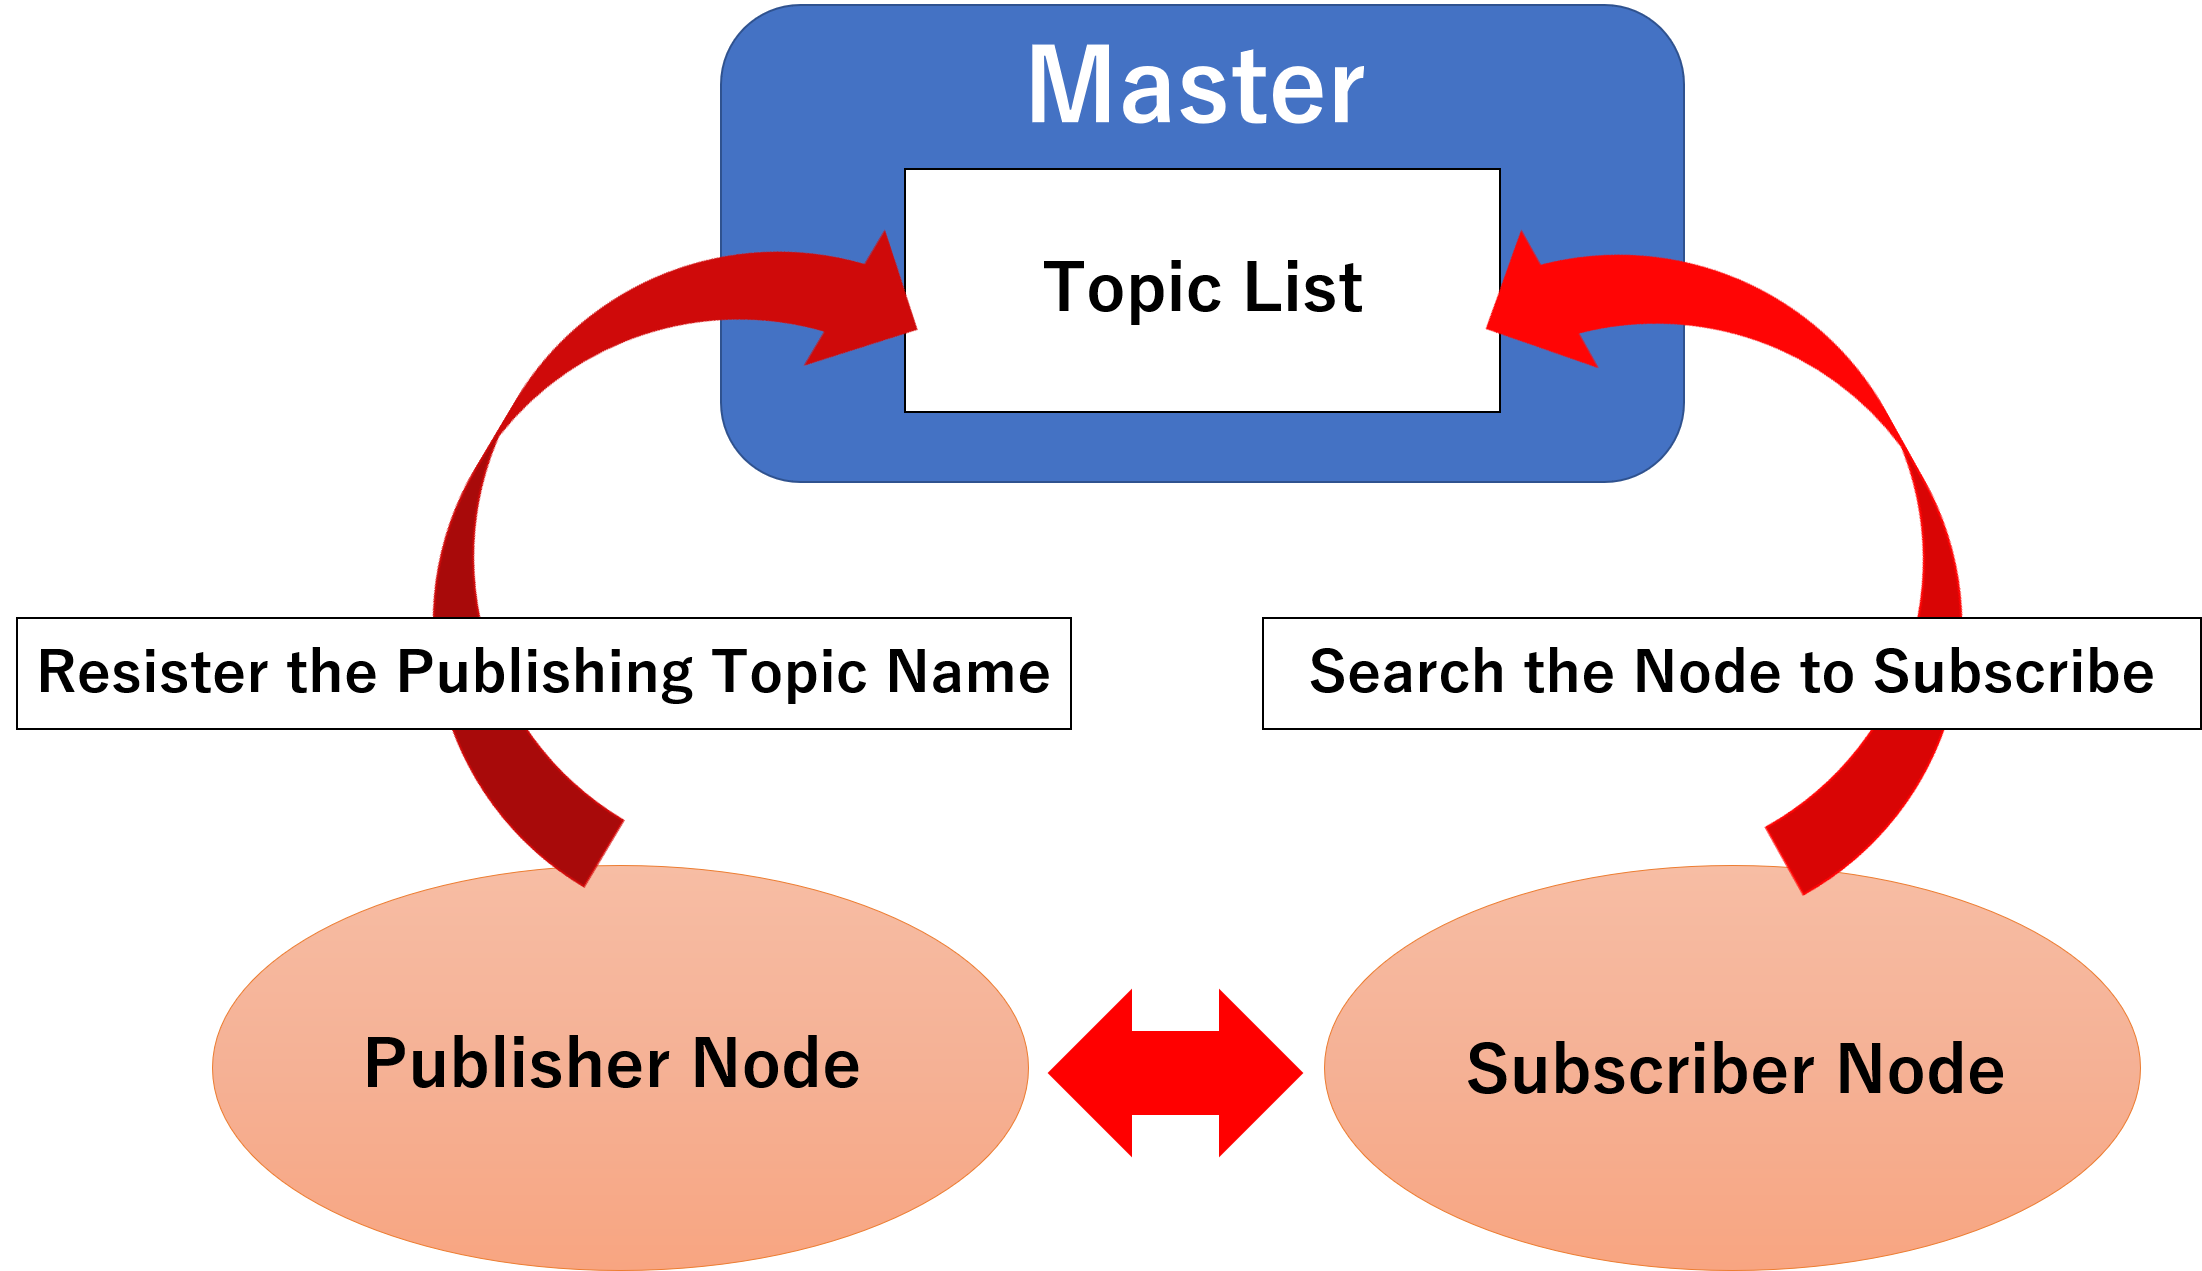
\includegraphics[width=1.0\linewidth, clip]{./figure/chapter4/ros.png}
    \caption{ROS Communication Model}
    \label{fig:ros}
\end{figure}

\section{ROSによるUAV制御}
本研究では,撮影計画を実装するUAVとして,民生用ドローンおよび関連機器製造会社であるDJI社のMavic Miniを複数台使用する.
以下,MavicMiniの性能の概要と制御を行うための通信モデルについて説明する.

\begin{figure}[h]
    \centering
    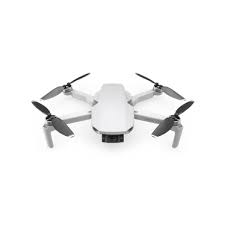
\includegraphics[width=0.7\linewidth, clip]{./figure/chapter4/mavic_mini.jpg}
    \url{Source:https://www.dji.com/jp/mavic-mini}
    \caption{Mavic Mini}
    \label{fig:mavic_mini}
\end{figure}

MavicMiniはGPSセンサを搭載しており,フライトコントローラで自身の位置情報を管理している.
昨年度まで使用していた同社が販売しているMatrice600とは異なり,ROSと直接通信ができるDJI Onboard SDKが使用できない.
そのためMavicMiniの制御はDJI Mobile SDKを用いて行う.
DJI Mobile SDKはAndroid端末,IOS端末のアプリによりフライトコントローラとROSの通信を可能にするAPIを提供する.
今回の実験ではAndroid端末でMavicMiniを制御するアプリを開発し,無線LANによってROSマスターと通信を行う.
図に通信モデルを示す.



\section{地上設置LiDARとGPSセンサ}
LiDARはレーザ機器やセンサなどの開発を行う北陽電機株式会社のUTM-30LX-EW,同社のUST-30LXの2台を使用する.
性能はどちらも検出範囲は270[deg],角度分解能は0.25[deg]であり,LANケーブルから点群情報を送信する.

\begin{figure}[b]
    \centering
    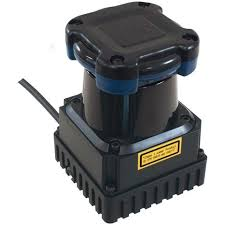
\includegraphics[width=0.5\linewidth, clip]{./figure/chapter4/lidar1.jpg}
    \url{Source:https://www.hokuyo-aut.co.jp/search/single.php?serial=146}
    \caption{UTM-30LX-EW}
    \label{fig:lidar1}
\end{figure}

\begin{figure}[t]
    \centering
    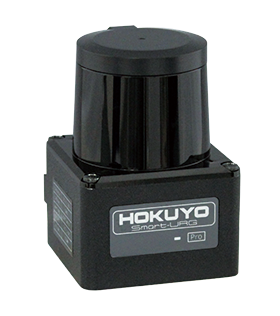
\includegraphics[width=0.5\linewidth, clip]{./figure/chapter4/lidar2.png}
    \url{Source:https://www.hokuyo-aut.co.jp/search/single.php?serial=195}
    \caption{UST-30LX}
    \label{fig:lidar2}
\end{figure}

本研究では3章で示した通り,LiDARの位置情報をGPSセンサから取得し,map座標を得る.
今回の実験ではGPSセンサはublox社のマルチバンドGNSSアンテナのANN-MB-01を使用する.

\begin{figure}[h]
    \centering
    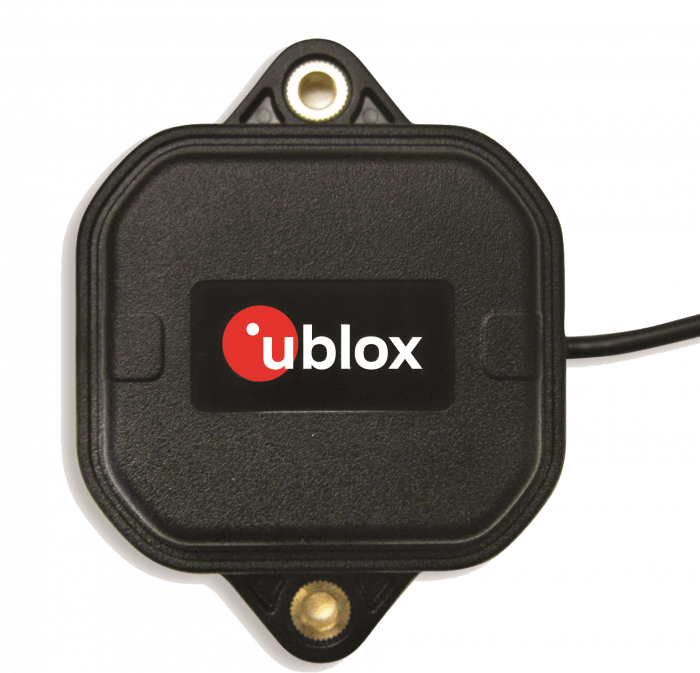
\includegraphics[width=0.5\linewidth, clip]{./figure/chapter4/GPS.png}
    \url{Source:https://www.hokuyo-aut.co.jp/search/single.php?serial=146}
    \caption{Multi-band GNSS Antenna ANN-MB-01}
    \label{fig:GPS}
\end{figure}

昨年度の研究ではLiDARの情報を有線LANケーブルでホストPCに送信していたが,
LiDARを複数台使用する場合,有線LANケーブルで接続するのは非常に不便であり効率が悪い.
そこで,LiDARの点群情報とGPSセンサからの位置情報を無線でホストPCに送信するシステムを構築する,
LiDARやGPSセンサから直接データを無線通信することができないので,
一旦ホストPCとは別のPCに接続してそのPCからホストPCへ無線接続する.
LiDARと接続するPC(サブPC)にはRaspberry Pi4 modelBを採用した.Raspberry Pi4はUbuntu server OS
に対応しておりROSをインストールすることができる.
LiDARをサブPCに有線LANケーブルで接続し,サブPC内で点群情報をROSトピックとして配信する
ノードを立ち上げることでホストPCとの無線接続を可能とする.
GPS情報はサブPCにデータを取り込んだ後,サブPCとホストPCでTCP通信を行う.
ホストPCで,受け取ったGPS情報をトピックに変更するノードを立ち上げることにより,LiDARの位置情報を
UAV撮影計画のROSプログラム内で使用することができる.

\begin{figure}[h]
    \centering
    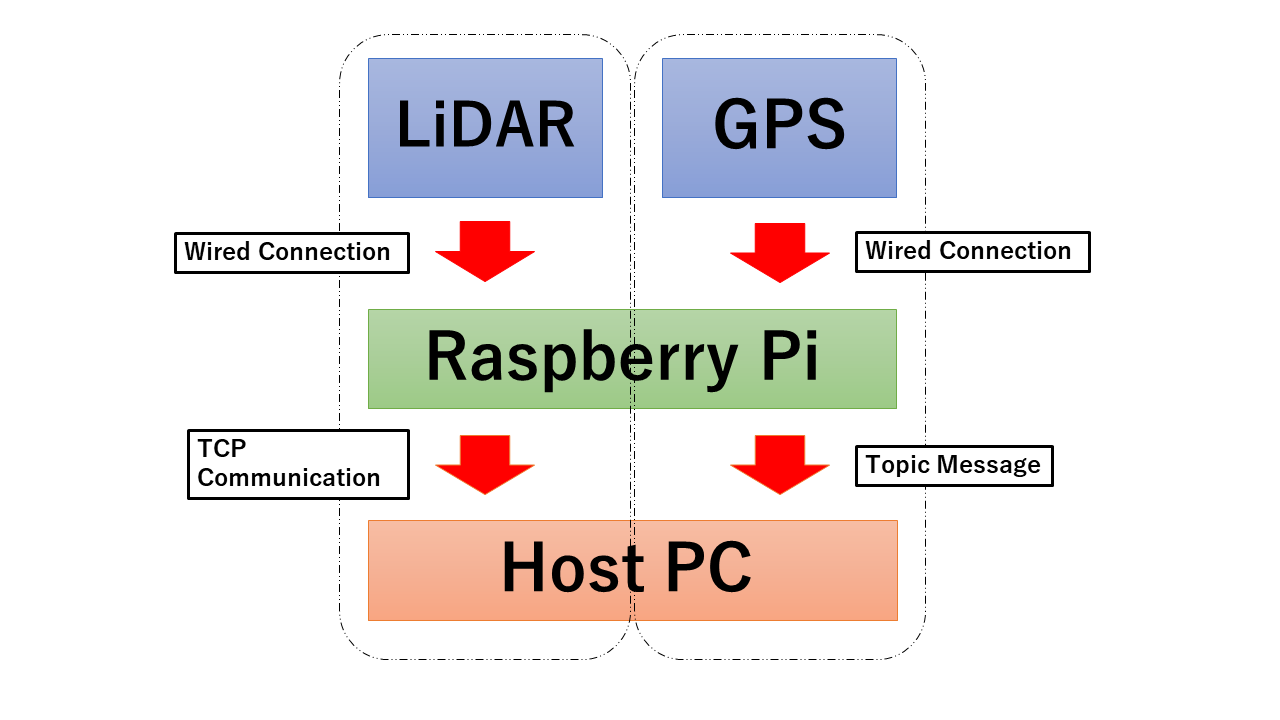
\includegraphics[width=1.0\linewidth, clip]{./figure/chapter4/wireless_model.png}
    \caption{Wireless Communication Model for LiDAR and GPS antenna}
    \label{fig:wireless_model}
\end{figure}

\cref{fig:wireless_model}はLiDAR周りの通信モデルである.

\cref{fig:system}にこのシステム全体の通信モデルを示す.
赤で示されている通信が無線通信であり,水色で示されている通信が有線通信である.

\newpage
\begin{figure}[h]
    \centering
    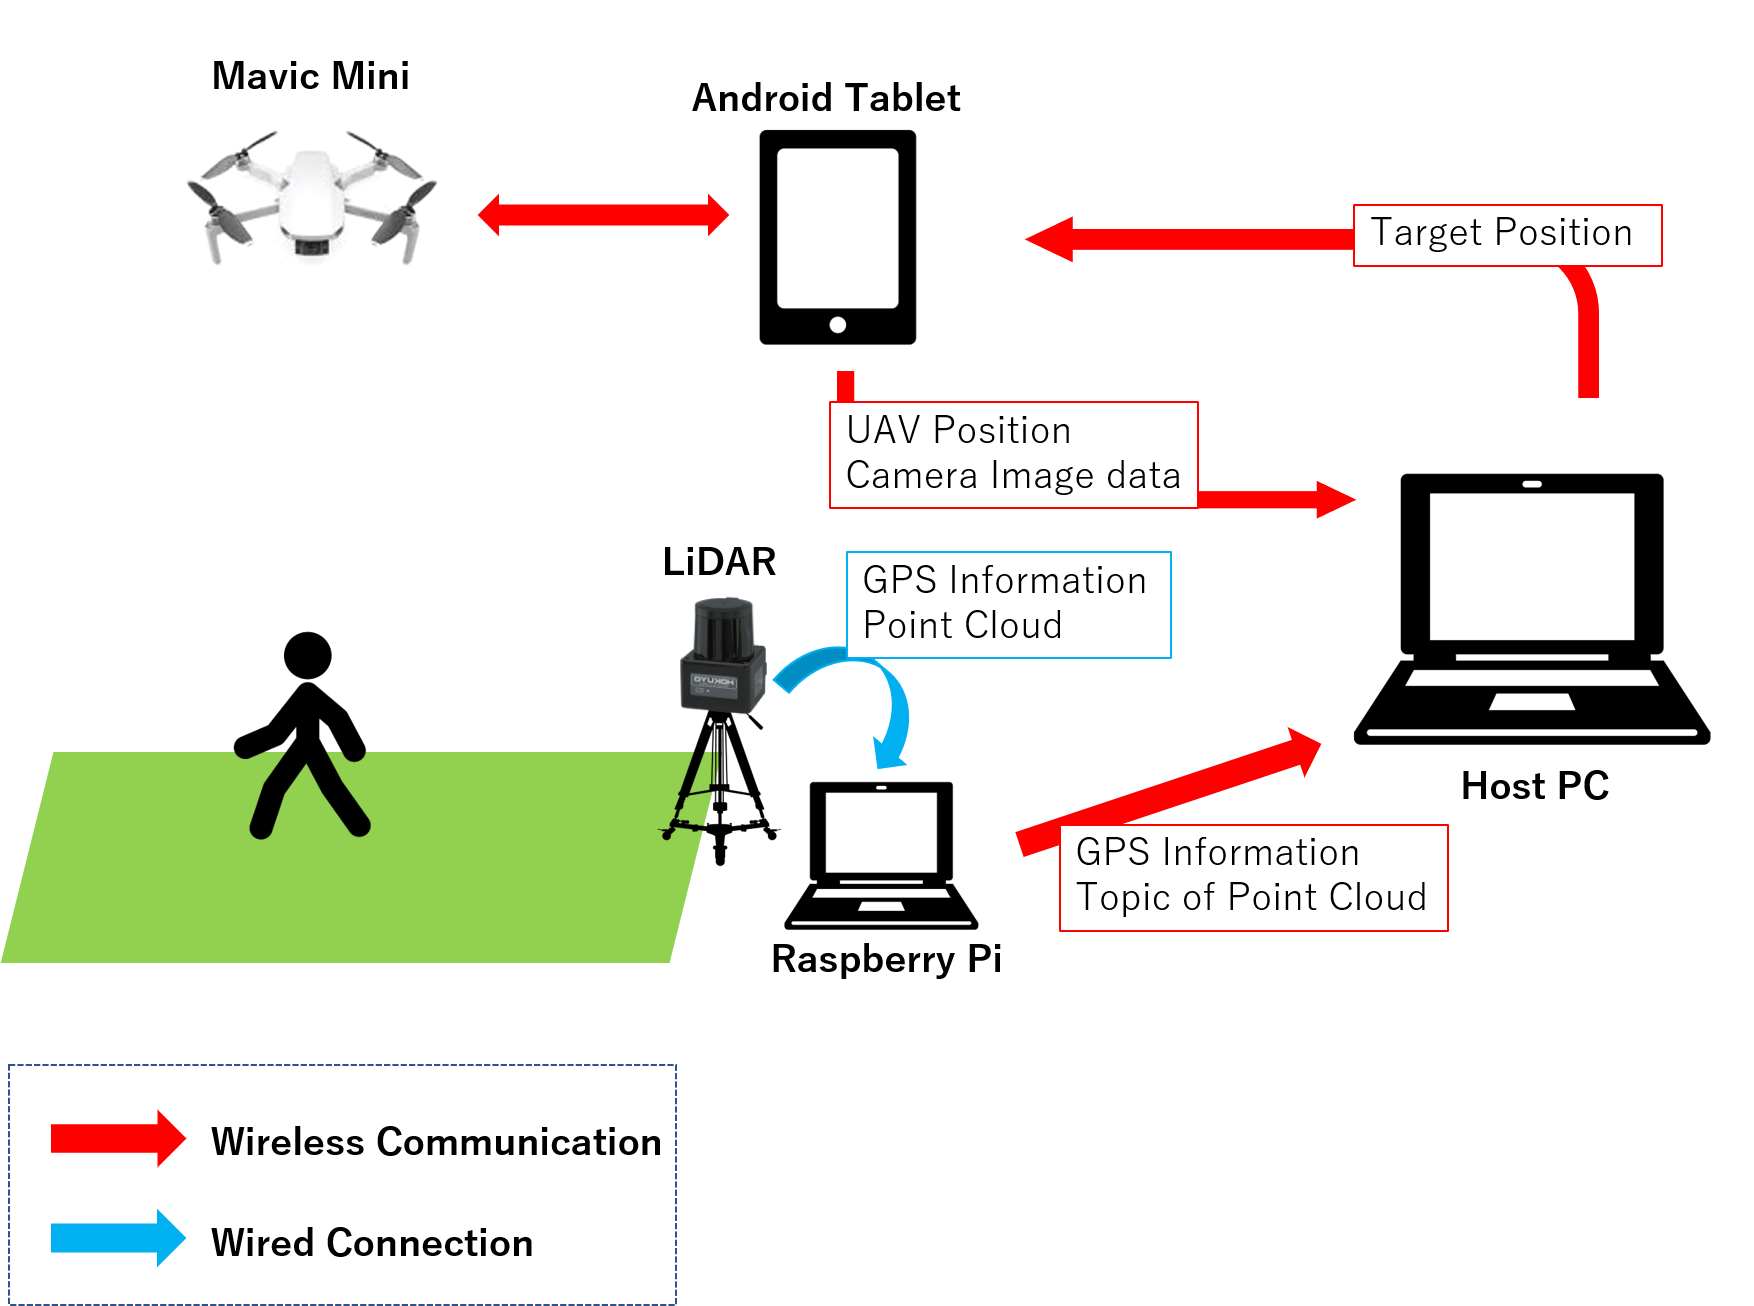
\includegraphics[width=0.8\linewidth, clip]{./figure/chapter4/communication_model.png}
    \caption{Communication System}
    \label{fig:system}
\end{figure}


\newpage
\section{本章のまとめ}
本章では,2章で説明した撮影計画および人物検出,また3章で説明した複数台LiDARの設置方法およびダミー人物の設定
方法を実装したシステムについて説明した.
次章では,本章で説明したシステムを利用して,実環境において複数人物の追従と撮影計画を行った実験について述べる.

\end{document}
